\section*{Kinetics, Constitutive Laws, and Viscoelasticity I}

\subsection*{2--1. \textbf{Balance of mass} [4 pts].} 
A large piece of polydimethylsiloxane (PDMS) of uniform density $\rho(\bm{x},t)$ has a central spherical bubble of time-evolving radius $R(t)$, initial radius $R_0$, and wall velocity of $\dot{R}$. 
The hole is subject to a uniform surface traction in the $\bm{e}^{(r)} \equiv \bm{e}_{\bm{r}}$ direction from an axisymmetric pressure, and maintains spherical symmetry over time. 

\medskip
The position of a point in the material can be written as $\bm{x} = r(R,t) \bm{e}_{\bm{r}}$ with reference position $\bm{X} = r_0(R_0)$, while the velocity of that point can be written as $\bm{v}(r,t) = v_r \bm{e}_{\bm{r}}$.

\medskip
Using the conservation of mass equation, show that the material must satisfy
%\begin{equation}
%\rho_{,t} + (\rho v_i)_{,i} = 0,
%\end{equation}
\begin{equation*}
\rho_{,t}+ \rho_{,r} v_r + \frac{\rho}{r} (v_r + r v_{r,r}) = 0,
\end{equation*}
and hence, show that an assumption of incompressibility for PDMS results in 
\begin{equation*}
v_r(r,t) = \frac{R^2 \dot{R}}{r^2}.
\end{equation*}

\medskip
\subsection*{2--2. \textbf{Balance of momenta} [4 pts].} A spherical hydrogel body $\mathcal{B}$ with a linear density gradient is currently submerged in water as depicted in the figure. 
The sphere has coordinates $\bm{x}$ in a region $\Omega$ with position-dependent density $\rho(\bm{x})$. 

\begin{figure}[H]
\vspace{-2em}
\centering
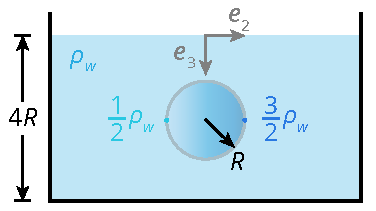
\includegraphics[width=3in]{instr-figures/PS2-Q1.pdf}
\caption{\small{Hydrogel sphere with a linear density gradient submerged in water. The water has a density $\rho_w$, while the sphere has a density at its leftmost point of $\rho_w/2$ and at its rightmost point of $3\rho_w/2$.}}
\end{figure}

\vspace{-1em}
The surface traction $\bm{t}(\bm{x},\hat{\bm{n}})$ acting on $\mathcal{B}$ is given by 
\begin{equation*}
\bm{t}(\bm{x},\hat{\bm{n}}) = -\rho_w g x_3 \hat{\bm{n}},
\end{equation*}
where $\hat{\bm{n}}$ is the outer unit normal to the surface $\partial \Omega_t$ and $\rho_w$ is the (constant) density of water and $g$ is the acceleration due to gravity. 

\medskip
(a) Determine the net force and moment acting on $\mathcal{B}$ via volume integrals.

\medskip
(b) Under what \textit{two} conditions is $\mathcal{B}$ in static equilibrium?

\bigskip
\subsection*{2--3. \textbf{Viscoelastic data} [4 pts].} 
Stress relaxation isochrones for a compliant viscoelastic material are shown in the figure below.  

\begin{figure}[H]
\vspace{-1em}
\centering
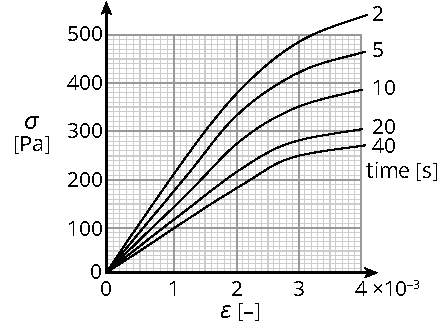
\includegraphics[scale = 1.5]{instr-figures/PS2-Q3.pdf}
\caption{\small{Stress (Pa) vs. strain ($-$) for a soft viscoelastic material.}}
\end{figure}

\vspace{-1em}
(a) Are these isochrones from a material which we can describe with linear viscoelasticity? If not, why not, and if so, under what approximate regimes would this assumption be valid? 

\medskip
(b) Estimate the creep relaxation function $J_c$ for stress values of 100 and 250 kPa. Isochrones are shown at times of 2, 5, 10, 20, and 40 seconds.   
% This is a placeholder for the example problems from the second problem set. 
% You'll replace this file with the one I supply on canvas. 

\bigskip
\subsection*{2--4. \textbf{Impulsive stresses} [4 pts].}

(a) Say that instead of a step load, we apply $\sigma(t) = A \delta(t)$ to an unknown linear viscoelastic material. 
Determine the strain history $\epsilon(t)$, first as a general function of the creep relaxation function $J_c(t)$, and then for a Kelvin-Voigt solid. 

(b) Now, consider a rapid load followed by a rapid reverse load by applying a doublet function of stress, i.e. $\sigma(t) = B \psi(t)$. 
What is the strain function $\epsilon(t)$ in terms of $J_c(t)$ and for a Kelvin-Voigt material now? 

\bigskip
\subsection*{2--5. \textbf{Two-element models} [8 pts].}

Dynamic mechanical analysis (DMA) is a common technique for characterizing viscoelasticity. 
DMA conventionally involves application of a sinusoidal displacement to the top surface of a sample at a controllable temperature. 
Often, the user puts the sample into initial compression, and follows with the sinusoidal profile. 
A cylindrical sample of height $h$ and diameter $d$ is placed between two plates.
The DMA then quickly puts the sample into compression by moving its top plate downward by a displacement $d$, and then oscillates sinusoidally between positions $0$ and $2d$ at a frequency $\omega$.

\medskip
(a) Using the constitutive law for a Kelvin-Voigt material, determine the stress $\sigma(t)$ exerted by the platens to cause the applied strain. 

\medskip
(b) The resulting stress lags behind the strain by an phase $\delta$, as in $\sin(\omega t + \delta)$. 
Commonly this is reported as the ``tangent loss", or $\tan\delta$, for a material. 
What is the value of $\tan\delta$ for this particular Kelvin-Voigt model?

\medskip
(c) Say instead of prescribing the strain $\epsilon(t)$, we instead prescribed the stress, $\sigma(t) = - \sigma_0 - \sigma_0 \sin(\omega t)$. 
Determine the strain $\epsilon(t)$ for this prescribed stress.

\medskip
(d) Prove that the tangent loss function $\tan\delta$ is identical between the two loading methods.